\documentclass[11pt, oneside]{article} 
\usepackage{geometry}
\geometry{letterpaper} 
\usepackage{graphicx}
	
\usepackage{amssymb}
\usepackage{amsmath}
\usepackage{parskip}
\usepackage{color}
\usepackage{hyperref}

\graphicspath{{/Users/telliott_admin/Tex/png/}}
% \begin{center} 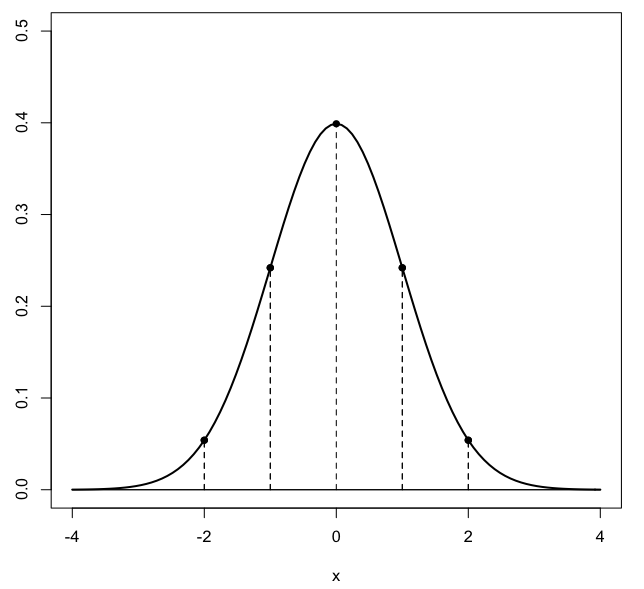
\includegraphics [scale=0.4] {gauss3.png} \end{center}

%break
\title{Parametrization}
\date{}

\begin{document}
\maketitle
\Large
The topic of parametrization (more rarely called parameterization) is a powerful abstraction.

Probably the simplest example is to describe motion in the plane using a single variable, often called $t$, because it can stand in for the time.

We can write
\[ x = f(t), \ \ \ \ y = g(t) \]
or more simply
\[ x = x(t), \ \ \ \ y = y(t) \]
or even
\[ \mathbf{r} = \langle x(t), y(t) \rangle \]

As the variable $t$ goes between some bounds, the vector $\mathbf{r}$ traces out a curve in the plane.  The essential reason that one variable can generate a curve is that the curve is one-dimensional, even though it "lives" in $\mathbb{R}^2$.

Examples include the circle of radius $r$
\[ \mathbf{r} = r \langle \cos t, \sin t \rangle \]
and the ellipse
\[ \mathbf{r} = r \langle a \cos t, b \sin t \rangle \]
In $\mathbb{R}^3$ we might make a spiral
\[ \mathbf{r} = r \langle a \cos t, b \sin t, t\rangle \]

For a region in the plane, we need two variables.  We have often used $x$ and $y$, and now more and more we use $r$ and $\theta$.  For example a region parametrized by $r,\theta$ could have area
\[ S(r, \theta) = \int_{\theta_1}^{\theta_2} \int_{r_1}^{r_2} \ dS  \]

By careful analysis and remembering that "area is length times length and an angle is not a length" we learned that the area element in polar coordinates is
\[ dA = dr \ \cdot r \ d \theta \]
usually written
\[ = r \ dr \ d \theta \]

A more formal statement is that the area elements in terms of $x,y$ ($dA = dx \ dy$) are related to those in terms of $r,\theta$  ($dS = dr \ d \theta$) by the Jacobian
\[ dA = J  \ dS \]
where
\[ J = | \ x_r y_{\theta}  - x_{\theta} y_r \ | \]

Since 
\[ x = r \cos \theta \]
\[ x_r = \cos \theta, \ \ \ x_{\theta} = - r \sin \theta \]
and
\[ y = r \sin \theta \]
\[ y_r = \sin \theta, \ \ \ y_{\theta} = r \cos \theta \]
we have
\[ J = | \ r \cos^2 \theta  + r \sin^2 \theta \ | = r \]
\[ dA = J \ dS = r dS \]
\[ dx \ dy = r \ dr \ d \theta \]

Other examples in $\mathbb{R}^2$ include the surface of a cylinder, parametrized by $(z,\theta)$ with constant radius $r$, and the surface of a sphere, parametrized by $(\phi,\theta)$ with constant radius $\rho$.  For the latter, the surface area is
\[ S = \int dS = \rho^2 \int_0^{2 \pi} \int_0^{\pi} \sin \phi \ d \phi \ d \theta \]
\[ = 4 \pi \rho^2 \]

We can also consider changes of coordinates.  A key feature is that we require area elements (with the appropriate Jacobian) and lengths to be invariant.

See the chapters on surface area and change of variables for details.

We can go on to $\mathbb{R}^3$, but I would rather look at examples of surfaces parametrized by two variables.  

To get the surface area of a solid whose surface is parametrized by $u,v$ we simply integrate
\[ S = \iint f(u,v) \ du \ dv \]
where for the area $f(u,v) = 1$.  We can use Fubini's theorem to write
\[  \iint \ du \ dv = \iint \ dv \ du \]
(with certain restrictions).  And as usual, while the outer integral covers the whole range of that variable, the interval for the inner variable may depend on the outer variable.

Here is an example from the web:

\url{http://mathinsight.org/parametrized_surface_area_examples}

\begin{center} 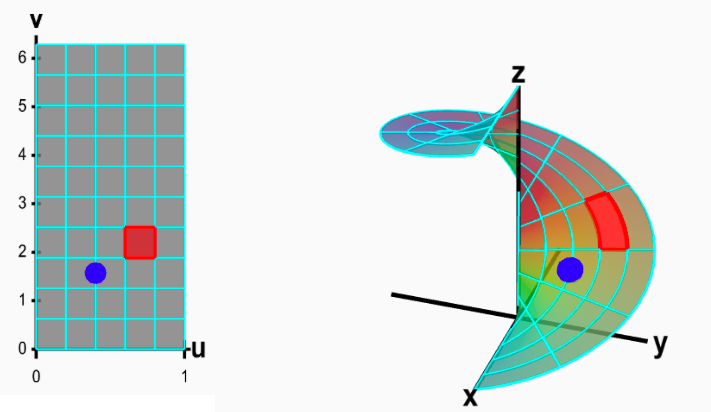
\includegraphics [scale=0.4] {helicoid.png} \end{center}

We stretch the rectangle on the left to be a helicoid on the right.  It can be parametrized as
\[ \mathbf{\Phi}(r,t) = (r \cos t, r \sin t, t) \] 
where now $r$ is not constant but a variable.  The region can be written
\[ D = [0,1] \times [0, 2 \pi] \]

To get the area we take the partial derivatives:
\[ \mathbf{\Phi}_r = \cos t, \sin t, 1 \]
\[ \mathbf{\Phi}_t = -r \sin t, r \cos t, 0 \]

The Jacobian is the absolute value of the cross-product:
\[ J = | \ (-r \cos t) \mathbf{\hat{i}} - (- r \sin t) \mathbf{\hat{j}} + (r \cos^2 t + r \sin^2 t) \mathbf{\hat{k}} \ | \]
\[ = \sqrt{r^2 \cos^2 t + r^2 \sin^2 t + r^2} \]
\[ = \sqrt{2r^2} = \sqrt{2} \ r \]

The area is then
\[ A = \int_0^{2 \pi} \int_0^1 J \ dr \ dt \]
$r$ and $t$ are independent so
\[ = 2 \pi \int_0^1 \sqrt{2} \ r \ dr\]
\[ = 2 \pi \sqrt{2} \  \int_0^1 r \ dr\]
\[ \pi r^2 \sqrt{2} \]

This is the area of an ellipse stretched in the $z$-direction,  Its projection in the plane is a circle.  Each little piece tilts up at an angle of 45 degrees.

\begin{center} 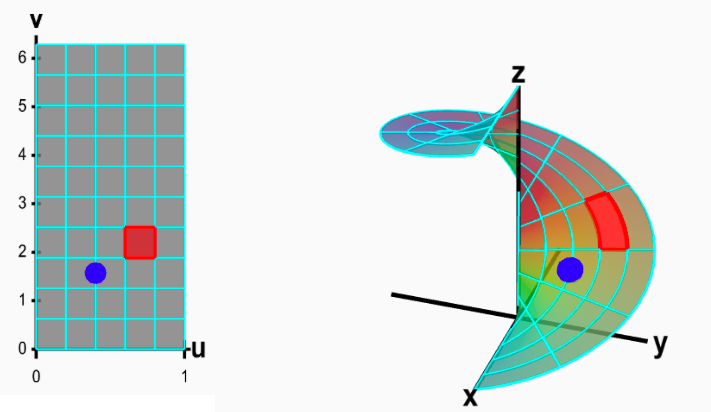
\includegraphics [scale=0.4] {helicoid.png} \end{center}

Seeing this as a tilted ellipse is a really interesting viewpoint.

\subsection*{Jacobian}

We've seen that the area element in polar coordinates is
\[ r \ dr \ d \theta \]

and the volume element in spherical coordinates is
\[ dV = \rho^2 \sin \phi  \ d \rho \ d \phi \ d \theta \]
We want to develop this in a more systematic way.

\subsection*{Ellipse}
Let's think about a standard ellipse
\[ \frac{x^2}{a^2} + \frac{y^2}{b^2} = 1 \]
Following the examples in the previous chapter, we might think about trying to compute the area of this ellipse as follows
\[ A = \iint\limits_{R} 1 \ dA = \iint\limits_{R} 1 \ dx \ dy \]
The problem is that we do not know how to specify the region for an ellipse, at least, not simply.  

However, a little trick can make that problem go away!

We will change both the horizontal and vertical dimensions by constant factors (different for $x$ and $y$).  We compress --- well, the opposite of stretching --- $x$ by the factor $1/a$ and similarly compress $y$ by the factor $1/b$.  We do this by making a change of variables
\[ x = au\] 
\[ dx = a\ du \]

\[ y = bv \]
\[ dy = b\ dv \]
So 
\[ dx \ dy = ab \ du \ dv \]
Substituting
\[ \frac{(au)^2}{a^2} + \frac{(bv)^2}{b^2} = u^2 + v^2 = 1\]
The substitution has converted the ellipse into a circle of radius $1$ and area $A = \pi$.
and
\[ A = \iint\limits_{R} 1 \ dx \ dy =  \iint\limits_{R} ab \ du \ dv \]
\[ = ab \iint\limits_{R} 1 \ du \ dv \]
Now, we know the area of the region in $u,v$ coordinates, it is a circle of radius $1$ and its area is just equal to $\pi$.  So finally
\[ A = ab \iint\limits_{R} 1 \ du \ dv = \pi a b \]

This is a really simple, beautiful result.  The two copies of $r$ in the formula $A= \pi r^2$ become $a \times b$.  Both dimensions make equivalent contributions to the area, as we'd expect.

The more formal way to do this is to compute what's called the Jacobian.  It gives the ratio between areas determined in two different coordinate systems.  We take the partial derivatives of $x$ with respect to $u$ and $v$, and similarly for $y$.
\[ x_u = a \]
\[ x_v = 0 \]
\[ y_u = 0 \]
\[ y_v = b \]

The two partials ($x_v$ and $y_u$) are zero because $x$ does not depend on $v$ and  $y$ does not depend on $u$.

We evaluate the determinant of this matrix:
\[ J = 
\begin{vmatrix}
x_u & x_v \\
y_u & y_v 
\end{vmatrix} =
\begin{vmatrix}
a & 0 \\
0 & b
\end{vmatrix} =ab
\]
If necessary, we take its absolute value.  And that's the factor for converting between the two coordinate systems.

Sometimes the Jacobian is written as
\[ J = 
\begin{vmatrix}
x_u & y_u \\
x_v & y_v 
\end{vmatrix}
\]
but this doesn't change anything, because $det(A) = det(A^T)$.

To summarize:
\[ dx \ dy = J \ du \ dv \]
where
$J$ is computed as described.

\section*{Circle}
The Jacobian is done like this: 
\[ x = r \cos \theta \]
\[ y = r \sin\ \theta \]

We compute
\[ x_r = \frac{\partial x}{\partial r} = cos \ \theta \]
\[ x_{\theta} = \frac{\partial x}{\partial \theta} = -r \ sin \ \theta \]
and similarly for $y$.  Then
\[ J = 
\begin{vmatrix}
x_r & x_{\theta} \\
y_r & y_{\theta} 
\end{vmatrix} =
\begin{vmatrix}
\cos\ \theta & -r \ sin\ \theta \\
\sin\ \theta & r \ cos\ \theta 
\end{vmatrix} = r (cos^2\ \theta + sin^2\ \theta) = r
\]
This is the factor for the ratio of areas under the two systems, and that's why we have $r\ dr \ d\theta$ in the integral.  Notice that when we took the partial derivatives, they were partials of $x,y$ with respect to $r,\theta$, and we end up multiplying $dr \ d\theta$ by J.

\end{document}